% !TEX TS-program = pdflatex
\documentclass[11pt]{article}

% ---------- Preamble ----------
\usepackage[a4paper,margin=1in]{geometry}
\usepackage[T1]{fontenc}
\usepackage[utf8]{inputenc}
\usepackage{lmodern}
\usepackage{microtype}

\usepackage{amsmath,amssymb,mathtools}
\usepackage{physics}
\usepackage{bm}
\usepackage{siunitx}

\usepackage{graphicx}
\usepackage{subcaption}
\usepackage{booktabs}
\usepackage{enumitem}
\usepackage{xcolor}
\usepackage{hyperref}
\usepackage[nameinlink]{cleveref}

\usepackage{algorithm}
\usepackage{algpseudocode}

% Toggle: tech report vs blog
\newif\iftech
\techtrue   % <- set to \techfalse for a shorter, blog-style build

% Handy macros
\newcommand{\E}{\mathbb{E}}
\newcommand{\KL}{\mathrm{KL}}
\newcommand{\N}{\mathcal{N}}
\newcommand{\R}{\mathbb{R}}
\newcommand{\dataset}{\mathcal{D}}
\newcommand{\model}{\mathcal{M}}
\newcommand{\student}{S}
\newcommand{\teachers}{\{T_i\}_{i=1}^M}
\newcommand{\todo}[1]{\textcolor{red}{\textbf{TODO:} #1}}

% Meta
\title{Bensemble}
% \author{Your Name \and Your Collaborators}
\date{\year}

% ---------- Document ----------
\begin{document}
\maketitle

% ----- Abstract / Motivation -----
\begin{abstract}
We introduce Bensemble, a PyTorch library for Bayesian ensembling with optional Rényi-divergence–guided model selection and posterior estimation, covering Laplace, and PBP.
\end{abstract}

\section{Introduction}
Rapid progress in deep learning has set new accuracy records, but it has also revealed a gap between what models \emph{predict} and how \emph{certain} they are. Real systems operate under distribution shift, limited data, and changing costs of error, so we need predictions that come with reliable uncertainty.

At its core, \emph{Bayesian ensembling} treats model parameters as random rather than fixed, and forms decisions by averaging predictions across plausible models. This produces a \emph{posterior predictive} distribution that better reflects epistemic uncertainty and tends to calibrate confidence to reality.

Thus, we present our Python library \textbf{Bensemble} that makes Bayesian ensembling easy to use in PyTorch. The library centers on building posterior predictives through a simple interface for training, drawing model samples (or approximations) and combining them. We also expose a tunable $\alpha$-divergence (R\'enyi) objective to steer selection and aggregation.


\section{A short refresher on the Bayesian approach}
Let $\mathcal{D}$ be data and $w$ denote model parameters.
\begin{align}
\textbf{Posterior:}\quad & p(w \mid \mathcal{D}) \;\propto\; p(\mathcal{D}\mid w)\,p(w). \\
\textbf{Evidence:}\quad & p(\mathcal{D}) \;=\; \int p(\mathcal{D}\mid w)\,p(w)\,dw \quad. \\
\textbf{Predict:}\quad & p(y\mid x,\mathcal{D}) \;=\; \int p(y\mid x,w)\,p(w\mid \mathcal{D})\,dw.
\end{align}


\section{Package content.} 
Overview of modules and APIs: trainers, objectives, metrics (RMSE/LL/Brier) with common interfaces.  

\section{Implementation details.} 
Details on the code and structure. What and how to call and compute. 

\section{Demo.} 
Runnable example: single-network baseline $\rightarrow$ ensemble with methods in the package. We show RMSE, NLL, Brier.  
\begin{figure}
    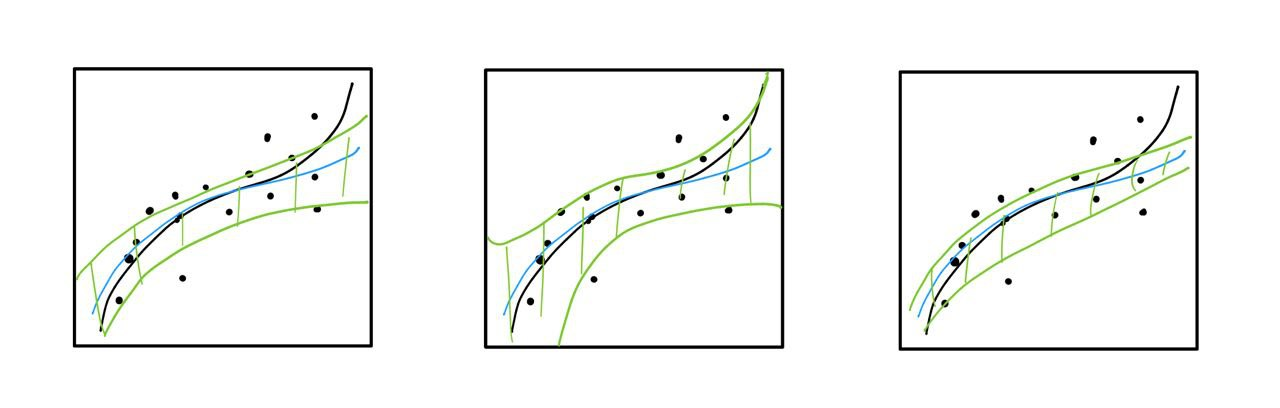
\includegraphics[width=1\textwidth]{example_graphs_bmm.jpg}
    \caption{Preliminary variant of the graph we want to include. We want to compare predictions of various methods.}
\end{figure}

\section{Conclusion.} 
Takeaways, when-to-use-what checklist, limitations (posterior misspecification, costs).

% \section{Introduction}
% Modern neural networks often achieve strong accuracy while drifting on confidence, especially under distribution shift or scarce data. \emph{Bayesian ensembling} counters this by maintaining (or approximating) a posterior over models and averaging predictions to form the posterior predictive, which typically improves calibration and surfaces epistemic uncertainty.

% We present \textbf{Bensemble}: a PyTorch library that unifies five practical routes to posterior samples---\textbf{VI/ELBO}, \textbf{scalable Laplace}, \textbf{HMC}, \textbf{MC Dropout}, and \textbf{Probabilistic Backpropagation (PBP)}---and augments them with \textbf{R\'enyi-divergence--guided selection and aggregation}. The tunable parameter $\alpha$ enables risk-sensitive control over how ensemble members are weighted, yielding practical trade-offs among calibration, NLL, and tail risk. The toolkit includes drop-in training/inference hooks, reliability metrics (ECE, Brier, NLL), and $\alpha$-sweep utilities to visualize the accuracy--uncertainty frontier as you vary sample count, curvature, or priors. In short, plug it into standard PyTorch workflows to obtain calibrated, uncertainty-aware predictions without heavy engineering overhead.


% \section{Quick theory on bayesian approach}
% Given data $\dataset=\{(x_n,y_n)\}_{n=1}^N$ and a model $m\in\model$ (e.g., network weights and hyperparameters), the posterior predictive is
% \begin{equation}
% p(y\mid x,\dataset)\;=\;\int p(y\mid x,m)\,p(m\mid\dataset)\,dm
% \quad\approx\quad \frac{1}{K}\sum_{k=1}^K p(y\mid x,m^{(k)}), 
% \end{equation}
% with $\{m^{(k)}\}$ drawn via an approximation method.
% Calibration improves when $p(m\mid\dataset)$ is captured broadly enough to reflect epistemic uncertainty.

% \section{Package content}
% Describe available methods. Add references to original papers. Add short theory describing each method. 

% \section{Implementation}
% Short description of package design, what we implemented. Maybe add how we implemented. 


% \section{Demo}
% Will add link to the demo code. From there we can show some numeric results. 

% \section{Conclusion}
% Words to conclude. Why our library is cool and why/when a reader should use it. 

\end{document}
